\graphicspath{{lab36/pic/}}

\chapter{实现一个ls命令}

\section{实验目的}
\begin{enumerate}
	\item 理解inode文件名的存储方式
	\item 学会添加一个新的系统调用
\end{enumerate}

\section{实验内容}
    \begin{enumerate}
        \item 在xtsh命令行中,实现一个类似Linux的ls命令,列出系统所有文件
    \end{enumerate}
\section{预备知识}

本实验基于《操作系统设计与实现》教材中第八章《xtfs文件系统》和第十二章《文件操作》,写者需先掌握第八章基础知识,熟悉code8和code12。

\section{实验环境}

\begin{itemize}
	\item 操作系统:ubuntu20.04
	\item 虚拟机:qemu-system-loongarch64
\end{itemize}

\section{实验原理}
    \item 挂载时已把inode所有信息读取到inode\_table,遍历inode\_table即可

\section{实验步骤}
\begin{enumerate}
    \item 增加一个sys\_ls()函数,如下图
        \begin{figure}[H] 
            \centering 
            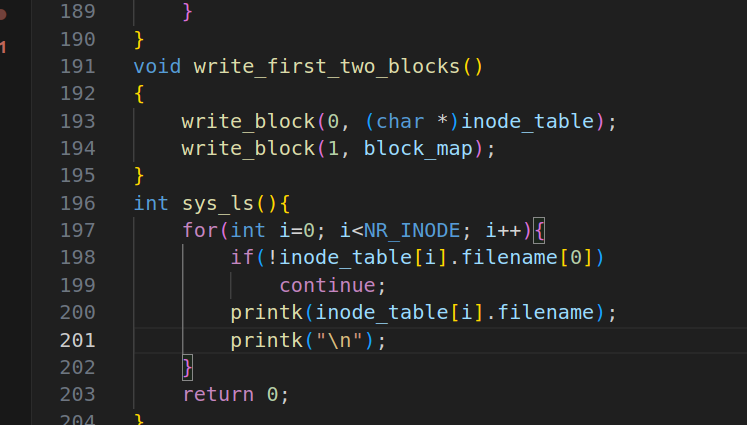
\includegraphics[width=0.5\textwidth]{lab36/pic/36.1.png}
            \caption{sys\_ls函数} 
            \label{picture_name}
        \end{figure} 
	\item 编写可执行文件ls.S
        \begin{figure}[H] 
            \centering 
            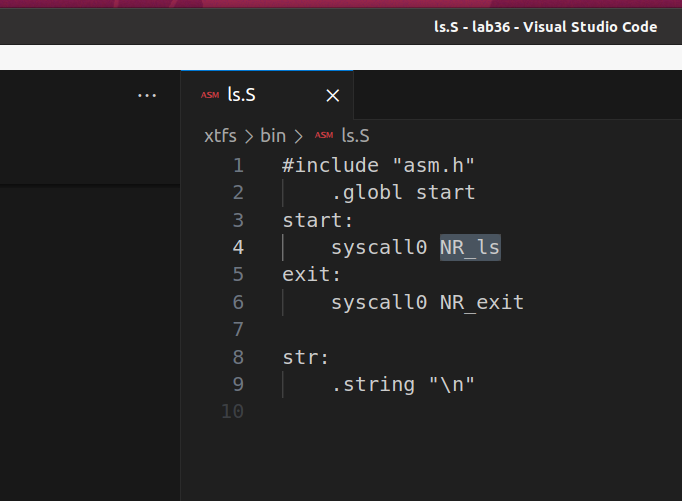
\includegraphics[width=0.5\textwidth]{lab36/pic/36.2.png}
            \caption{ls.S} 
            \label{picture_name}
        \end{figure}    
\end{enumerate}


\section{实验结果}
\begin{figure}[H] 
	\centering 
	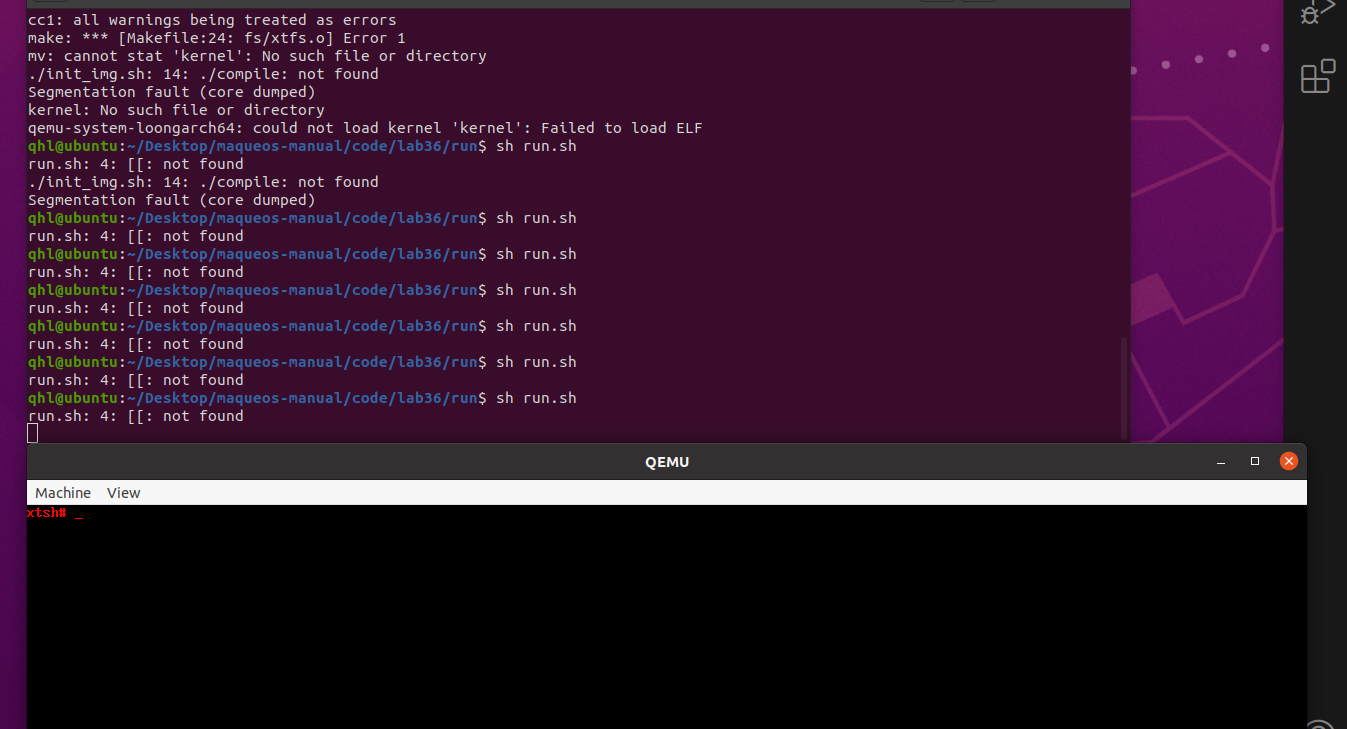
\includegraphics[width=0.5\textwidth]{lab36/pic/36.3.png}
	\caption{验证ls命令} 
	\label{picture_name}
\end{figure}
上图所示,ls列出了系统所有文件

\section{实验报告要求}
完成代码编写并检查无误后,应进行实验报告的撰写,要求对源码中做出的修改进行文字说明,并对实验结果进行展示。